\documentclass[a4paper, 12pt]{article}%тип документа

%отступы
\usepackage[left=1.5cm,right=1cm,top=2cm,bottom=3cm,bindingoffset=0cm]{geometry}
\setlength{\parindent}{5ex}

%Русский язык
\usepackage[T2A]{fontenc} %кодировка
\usepackage[utf8]{inputenc} %кодировка исходного кода
\usepackage[english,russian]{babel} %локализация и переносы

%Вставка картинок
\usepackage{graphicx}
\graphicspath{{pictures/}}
\DeclareGraphicsExtensions{.pdf,.png,.jpg,}
\usepackage{wrapfig}

%Графики
\usepackage{pgfplots}
\pgfplotsset{compat=1.9}

%Математика
\usepackage{amsmath, amsfonts, amssymb, amsthm, mathtools}

%Таблицы
\usepackage{longtable} 
\usepackage{float}

%Римские цифры
\newcommand{\RomanNumeralCaps}[1]{\uppercase\expandafter{\romannumeral#1}}

\usepackage{multirow}



\begin{document}
	\begin{titlepage}
		\begin{center}
			\textsc{Федеральное государственное автономное образовательное учреждение высшего образования«Московский физико-технический институт (национальный исследовательский университет)»\\[5mm]
			}
			
			\vfill
			
			\textbf{Отчёт по лабораторной работе 5.2.1\\[3mm]
				Опыт Франка-Герца
				\\[50mm]
			}
			
		\end{center}
		
		\hfill
		\begin{minipage}{.5\textwidth}
			Выполнил студент:\\[2mm]
			Сериков Василий Романович\\[2mm]
			группа: Б03-102\\[5mm]
			
		\end{minipage}
		\vfill
		\begin{center}
			Москва, 2023 г.
		\end{center}
		
	\end{titlepage}
	
	\newpage
	\setcounter{page}{2}
	\textbf{Аннотация}\\
	
	\textbf{Цель работы: }\\
Методом электронного возбуждения измерить энергии первого уровня атома гелия в динамическом и статическом режимах.\\

	\textbf{Теория}\\
Одним из простых опытов, подтверждающих существование дискретных уровней энергии атомов, является эксперимент Франка и Герца.

Разреженный одноатомный газ заполняет трехэлектродную лампу.  Электроны, испускаемые разогретым катодом, ускоряются в постоянном электрическом поле, созданным между катодом и сетчатым анодом лампы. Передвигаясь от катода к аноду, электроны сталкиваются с атомами гелия. Если энергия электрона, налетающего на атом, недостаточна для того, чтобы перевести его в возбуждённое состояние (или ионизовать), то возможны только упругие соударения, при которых электроны почти не теряют энергии, так как их масса в тысячи раз меньше массы атомов.

При увеличении напряжения на электродах увеличивается энергия электронов и оказывается достаточной для возбуждения атомов, при этом ток коллектора резко уменьшается. При дальнейшем увеличении потенциала анода ток коллектора возрастает, электроны, испытавшие неупругие соударения набирают энергию, достаточную для преодоления задерживающего потенциала.

\begin{figure}[H]
	\centering
	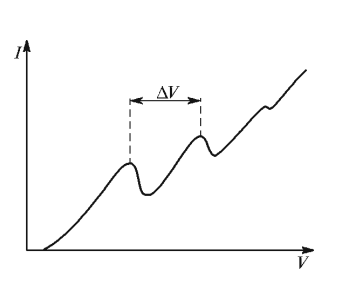
\includegraphics[width=0.6\linewidth]{1}
	\caption{Схематический вид зависимости тока коллектора от напряжения на аноде}
\end{figure}


\textbf{Экспериментальная установка}\\

Схема экспериментальной установки изображена на рис.2

Источником электронов является вольфрамовый катод, нагреваемы переменным током. В качестве анода используется двойная спираль, окружающая катод. Коллектор - полый цилиндр, соосный с катодом и анодом.  

\begin{figure}[H]
	\centering
	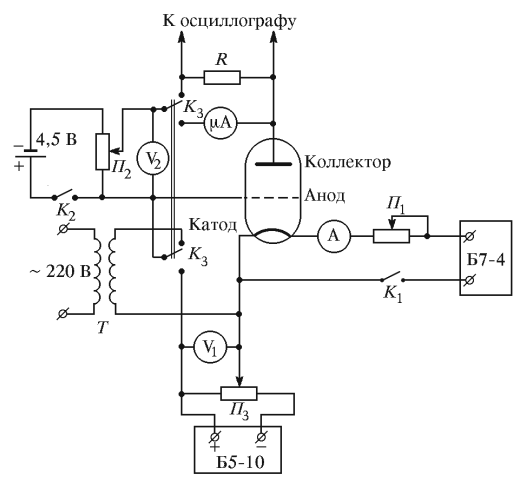
\includegraphics[width=0.6\linewidth]{ust}
	\caption{Схематический вид зависимости тока коллектора от напряжения на аноде}
\end{figure}




 
 
 \end{document}